%% (Master) Thesis template
% Template version used: v1.4
%
% Largely adapted from Adrian Nievergelt's template for the ADPS
% (lecture notes) project.


%% We use the memoir class because it offers a many easy to use features.
\documentclass[11pt,a4paper,titlepage]{memoir}

%% Packages
%% ========
%% LaTeX Font encoding -- DO NOT CHANGE
\usepackage[OT1]{fontenc}

%% Babel provides support for languages.  'english' uses British
%% English hyphenation and text snippets like "Figure" and
%% "Theorem". Use the option 'ngerman' if your document is in German.
%% Use 'american' for American English.  Note that if you change this,
%% the next LaTeX run may show spurious errors.  Simply run it again.
%% If they persist, remove the .aux file and try again.
\usepackage[english]{babel}

%% Input encoding 'utf8'. In some cases you might need 'utf8x' for
%% extra symbols. Not all editors, especially on Windows, are UTF-8
%% capable, so you may want to use 'latin1' instead.
\usepackage[utf8]{inputenc}

%% This changes default fonts for both text and math mode to use Herman Zapfs
%% excellent Palatino font.  Do not change this.
\usepackage[sc]{mathpazo}

%% The AMS-LaTeX extensions for mathematical typesetting.  Do not
%% remove.
\usepackage{amsmath,amssymb,amsfonts,mathrsfs}

%% NTheorem is a reimplementation of the AMS Theorem package. This
%% will allow us to typeset theorems like examples, proofs and
%% similar.  Do not remove.
%% NOTE: Must be loaded AFTER amsmath, or the \qed placement will
%% break
\usepackage[amsmath,thmmarks]{ntheorem}

%% LaTeX' own graphics handling
\usepackage{graphicx}

%% We unfortunately need this for the Rules chapter.  Remove it
%% afterwards; or at least NEVER use its underlining features.
\usepackage{soul}

%% This allows you to add .pdf files. It is used to add the
%% declaration of originality.
\usepackage{pdfpages}

%% Some more packages that you may want to use.  Have a look at the
%% file, and consult the package docs for each.
%% See the TeXed file for more explanations

%% [OPT] Multi-rowed cells in tabulars
%\usepackage{multirow}

%% [REC] Intelligent cross reference package. This allows for nice
%% combined references that include the reference and a hint to where
%% to look for it.
\usepackage{varioref}

%% [OPT] Easily changeable quotes with \enquote{Text}
%\usepackage[german=swiss]{csquotes}

%% [REC] Format dates and time depending on locale
\usepackage{datetime}

%% [OPT] Provides a \cancel{} command to stroke through mathematics.
%\usepackage{cancel}

%% [NEED] This allows for additional typesetting tools in mathmode.
%% See its excellent documentation.
\usepackage{mathtools}

%% [ADV] Conditional commands
%\usepackage{ifthen}

%% [OPT] Manual large braces or other delimiters.
%\usepackage{bigdelim, bigstrut}

%% [REC] Alternate vector arrows. Use the command \vv{} to get scaled
%% vector arrows.
\usepackage[h]{esvect}

%% [NEED] Some extensions to tabulars and array environments.
\usepackage{array}

%% [OPT] Postscript support via pstricks graphics package. Very
%% diverse applications.
%\usepackage{pstricks,pst-all}

%% [?] This seems to allow us to define some additional counters.
%\usepackage{etex}

%% [ADV] XY-Pic to typeset some matrix-style graphics
%\usepackage[all]{xy}

%% [OPT] This is needed to generate an index at the end of the
%% document.
%\usepackage{makeidx}

%% [OPT] Fancy package for source code listings.  The template text
%% needs it for some LaTeX snippets; remove/adapt the \lstset when you
%% remove the template content.
\usepackage{listings}
\lstset{language=TeX,basicstyle={\normalfont\ttfamily}}

%% [REC] Fancy character protrusion.  Must be loaded after all fonts.
\usepackage[activate]{pdfcprot}

%% [REC] Nicer tables.  Read the excellent documentation.
\usepackage{booktabs}


%% Our layout configuration.  DO NOT CHANGE.
%% Memoir layout setup

%% NOTE: You are strongly advised not to change any of them unless you
%% know what you are doing.  These settings strongly interact in the
%% final look of the document.

% Dependencies
\usepackage{ETHlogo}

% Turn extra space before chapter headings off.
\setlength{\beforechapskip}{0pt}

\nonzeroparskip
\parindent=0pt
\defaultlists

% Chapter style redefinition
\makeatletter

\if@twoside
  \pagestyle{Ruled}
  \copypagestyle{chapter}{Ruled}
\else
  \pagestyle{ruled}
  \copypagestyle{chapter}{ruled}
\fi
\makeoddhead{chapter}{}{}{}
\makeevenhead{chapter}{}{}{}
\makeheadrule{chapter}{\textwidth}{0pt}
\copypagestyle{abstract}{empty}

\makechapterstyle{bianchimod}{%
  \chapterstyle{default}
  \renewcommand*{\chapnamefont}{\normalfont\Large\sffamily}
  \renewcommand*{\chapnumfont}{\normalfont\Large\sffamily}
  \renewcommand*{\printchaptername}{%
    \chapnamefont\centering\@chapapp}
  \renewcommand*{\printchapternum}{\chapnumfont {\thechapter}}
  \renewcommand*{\chaptitlefont}{\normalfont\huge\sffamily}
  \renewcommand*{\printchaptertitle}[1]{%
    \hrule\vskip\onelineskip \centering \chaptitlefont\textbf{\vphantom{gyM}##1}\par}
  \renewcommand*{\afterchaptertitle}{\vskip\onelineskip \hrule\vskip
    \afterchapskip}
  \renewcommand*{\printchapternonum}{%
    \vphantom{\chapnumfont {9}}\afterchapternum}}

% Use the newly defined style
\chapterstyle{bianchimod}

\setsecheadstyle{\Large\bfseries\sffamily}
\setsubsecheadstyle{\large\bfseries\sffamily}
\setsubsubsecheadstyle{\bfseries\sffamily}
\setparaheadstyle{\normalsize\bfseries\sffamily}
\setsubparaheadstyle{\normalsize\itshape\sffamily}
\setsubparaindent{0pt}

% Set captions to a more separated style for clearness
\captionnamefont{\sffamily\bfseries\footnotesize}
\captiontitlefont{\sffamily\footnotesize}
\setlength{\intextsep}{16pt}
\setlength{\belowcaptionskip}{1pt}

% Set section and TOC numbering depth to subsection
\setsecnumdepth{subsection}
\settocdepth{subsection}

%% Titlepage adjustments
\pretitle{\vspace{0pt plus 0.7fill}\begin{center}\HUGE\sffamily\bfseries}
\posttitle{\end{center}\par}
\preauthor{\par\begin{center}\let\and\\\Large\sffamily}
\postauthor{\end{center}}
\predate{\par\begin{center}\Large\sffamily}
\postdate{\end{center}}

\def\@advisors{}
\newcommand{\advisors}[1]{\def\@advisors{#1}}
\def\@department{}
\newcommand{\department}[1]{\def\@department{#1}}
\def\@thesistype{}
\newcommand{\thesistype}[1]{\def\@thesistype{#1}}

\renewcommand{\maketitlehooka}{\noindent\ETHlogo[2in]}

\renewcommand{\maketitlehookb}{\vspace{1in}%
  \par\begin{center}\Large\sffamily\@thesistype\end{center}}

\renewcommand{\maketitlehookd}{%
  \vfill\par
  \begin{flushright}
    \sffamily
    \@advisors\par
    \@department%, ETH Z\"urich
  \end{flushright}
}

\checkandfixthelayout

\setlength{\droptitle}{-48pt}

\makeatother

% This defines how theorems should look. Best leave as is.
\theoremstyle{plain}
\setlength\theorempostskipamount{0pt}

%%% Local Variables:
%%% mode: latex
%%% TeX-master: "thesis"
%%% End:


%% Theorem environments.  You will have to adapt this for a German
%% thesis.
%% Theorem-like environments

%% This can be changed according to language. You can comment out the ones you
%% don't need.

\numberwithin{equation}{chapter}

%% German theorems
%\newtheorem{satz}{Satz}[chapter]
%\newtheorem{beispiel}[satz]{Beispiel}
%\newtheorem{bemerkung}[satz]{Bemerkung}
%\newtheorem{korrolar}[satz]{Korrolar}
%\newtheorem{definition}[satz]{Definition}
%\newtheorem{lemma}[satz]{Lemma}
%\newtheorem{proposition}[satz]{Proposition}

%% English variants
\newtheorem{theorem}{Theorem}[chapter]
\newtheorem{example}[theorem]{Example}
\newtheorem{remark}[theorem]{Remark}
\newtheorem{corollary}[theorem]{Corollary}
\newtheorem{definition}[theorem]{Definition}
\newtheorem{lemma}[theorem]{Lemma}
\newtheorem{proposition}[theorem]{Proposition}

%% Proof environment with a small square as a "qed" symbol
\theoremstyle{nonumberplain}
\theorembodyfont{\normalfont}
\theoremsymbol{\ensuremath{\square}}
\newtheorem{proof}{Proof}
%\newtheorem{beweis}{Beweis}


%% Helpful macros.
%% Custom commands
%% ===============

%% Special characters for number sets, e.g. real or complex numbers.
\newcommand{\C}{\mathbb{C}}
\newcommand{\K}{\mathbb{K}}
\newcommand{\N}{\mathbb{N}}
\newcommand{\Q}{\mathbb{Q}}
\newcommand{\R}{\mathbb{R}}
\newcommand{\Z}{\mathbb{Z}}
\newcommand{\X}{\mathbb{X}}

%% Fixed/scaling delimiter examples (see mathtools documentation)
\DeclarePairedDelimiter\abs{\lvert}{\rvert}
\DeclarePairedDelimiter\norm{\lVert}{\rVert}

%% Use the alternative epsilon per default and define the old one as \oldepsilon
\let\oldepsilon\epsilon
\renewcommand{\epsilon}{\ensuremath\varepsilon}

%% Also set the alternate phi as default.
\let\oldphi\phi
\renewcommand{\phi}{\ensuremath{\varphi}}


%% Make document internal hyperlinks wherever possible. (TOC, references)
%% This MUST be loaded after varioref, which is loaded in 'extrapackages'
%% above.  We just load it last to be safe.
\usepackage[linkcolor=black,colorlinks=true,citecolor=black,filecolor=black]{hyperref}

%% this is package for pseudocode
\usepackage{algorithm}
\usepackage{algpseudocode}

%% Document information
%% ====================

\title{Monocular Visual Odometry}
\author{Dongho Kang, Jaeyoung Lim, and Jihwan Youn}
\thesistype{Vision Algorithms for Mobile Robotics}
% \advisors{Advisors: Prof.\ Dr.\ Davide Scaramuzza}
% \department{}
\date{January 8, 2016}

\begin{document}

\frontmatter

%% Title page is autogenerated from document information above.  DO
%% NOT CHANGE.
\begin{titlingpage}
  \calccentering{\unitlength}
  \begin{adjustwidth*}{\unitlength-24pt}{-\unitlength-24pt}
    \maketitle
  \end{adjustwidth*}
\end{titlingpage}

%% The abstract of your thesis.  Edit the file as needed.
%\input{abstract}

%% TOC with the proper setup, do not change.
\cleartorecto
\tableofcontents
\mainmatter

%% Your real content!
% Some commands used in this file
\newcommand{\package}{\emph}

\setcounter{chapter}{-1}
\chapter{Instruction Manual}

\section{Environment}

\begin{figure}[h]
\centering
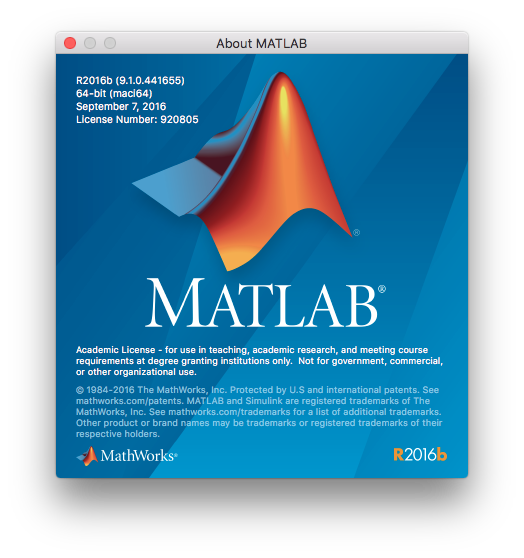
\includegraphics[width=0.6\textwidth]{aboutMatlab.png}
\caption{MATLAB Version Information (MATLAB for MAC OS X)}
\end{figure}

The code is written in Mathworks \textbf{\copyright MATLAB}. Due to the differences in several matrix operation, the code only works properly in \textbf{R2016b} version. Operating Systems of testing environments are \textbf{Linux Ubuntu 14.04 LTS} and \textbf{Apple Mac OS X El Capitan Version 10.11.6.}

We did not use any external libraries but only the modules developed during the exercises sessions and several MATLAB classes or functions which are allowed. (e.g. \textit{vision.PointTracker})

\section{Files}
\subsection*{Scripts}

.m script files are under \textit{src} directory. 

\begin{itemize}
\item \textit{main.m} \quad A main script for visual odometry pipeline. It invokes VO functions such as \textit{initializeVO, processFrame, bundleAdjustment} and \textit{visualizeFrame.} Also, it includes several running options such as choosing data set among KITTI / Malaga / Parking / Seoul and turn on/off features etc.

\item \textit{create\_bag.m} \quad This script generates bag of visual words and image index for each data set which can be used for image retrieve test and debug. Since place recognition does not work properly in our pipe line, it is deprecated now.
\end{itemize}

\subsection*{Visual Odometry Functions}

.m files below includes core logic of our VO pipeline. Please refer to \textbf{Monocular Visual Odometry} section for more details. Files are under \textit{src/visual\_odometry} directory.

\begin{itemize}
\item \textit{initializeVO.m} \quad Function for VO initialization operation.  
\item \textit{processFrame.m} \quad Function for VO continuous operation.
\item \textit{bundleAdjustment.m} \quad Function for bundle adjustment.
\item \textit{getParams.m} \quad This functions returns proper parameters for each data sets which were carefully chosen.
\item Functions for Loop Closure (\textit{./loopClosure\_sub}) 
\item Other sub-functions for functions above (\textit{./other\_sub})
\end{itemize}

\subsection*{Classes}

Class files are written in Object Oriented Programming style for containing data such as state, landmarks, candidates and parameter(\textit{Params\_XXX.m} files) They also includes several methods to process these data. Files are under \textit{src/class} directory.\newline \newline
Note: Please do not change value of parameter class properties. These values have been carefully chosen. 

\subsection*{Package Functions}

These .m files are developed during the exercise session. The files are under \textit{src/exercise\_packages} directory.

\subsection*{Files for Debugging}

These .mat files were used for debugging. It includes exported bag of visual words, image index etc. The files are under \textit{src/var\_debug} directory. \newline 
Note: For test VO, you do not need to concern about these files.

\subsection*{Data Set Files}

Data set files are images for VO pipeline. The files are under \textit{data} directory. \textbf{For submitted version, we included whole dataset files in the directory.} Please refer to \textbf{Installation and Running} section.

\begin{itemize}
\item KITTI \quad Path of the data set is \textit{data/kitti}  
\item Malaga \quad Path of the data set is \textit{data/malaga-urban-dataset-extract-07} 
\item Parking \quad Path of the data set is \textit{data/parking} 
\item Seoul \quad Data set which was created by us. It was generated from video recorded by iPhone 6 and processed (i.e. calibrated and rectified) using \href{https://www.vision.caltech.edu/bouguetj/calib_doc/}{MATLAB Camera Calibration Toolbox for MATLAB by Caltech.} Path of the data set is \textit{data/iphone} 
\end{itemize}



\section{Installation and Running}

We submit one .zip file which contains whole code and our own dataset. For a testing, extract the .zip file and please set dataset paths first, which defined in main script. Finally run \textit{main.m} script. \textit{main.m} automatically refer to other dependencies for running VO pipeline. 

Remark, our VO pipeline only works in \textbf{MATLAB R2016b} 

Note: Before run main script, \textbf{please check if you are in the \textit{src} directory.} In only works properly when work directory is \textit{src} directory. 


\chapter{Monocular Visual Odometry}\label{chap:initialization}
%In this section, we explain how we implemented our VO pipeline.

Our Visual Odometry pipeline(VO pipeline) consists of initialization, continuous operation, and bundle adjustment as shown in figure \ref{fig:overview}. A loop closure module was also implemented but excluded from the experimental result.

\begin{figure}[h] \label{fig:overview}
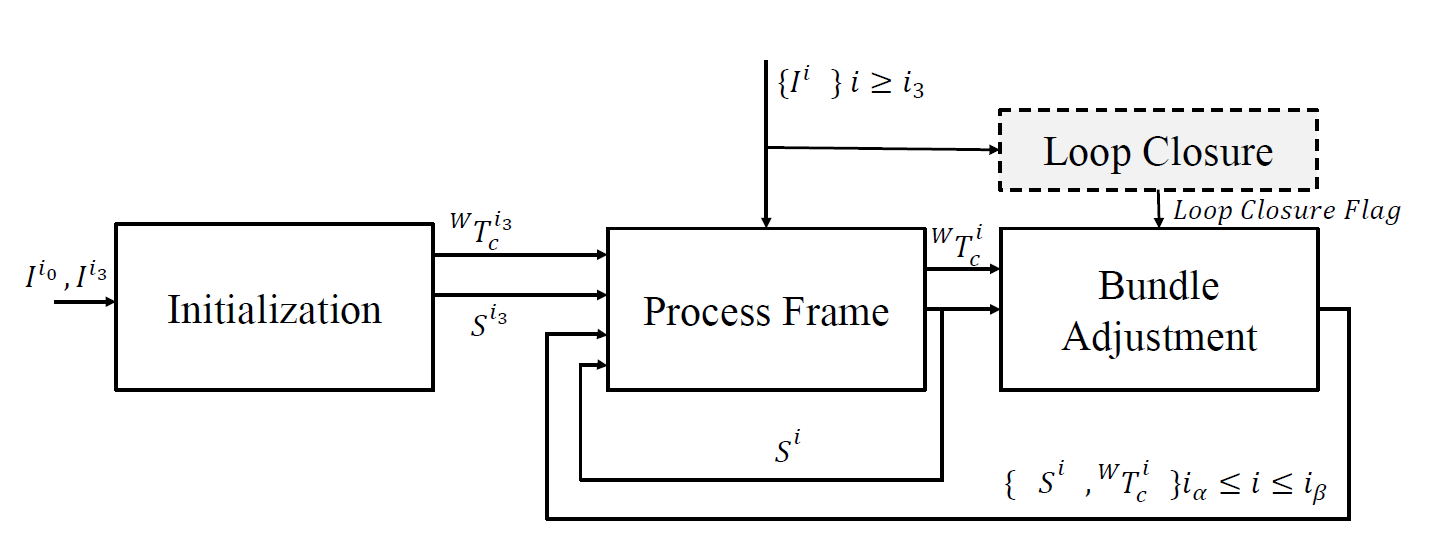
\includegraphics[width=\textwidth]{Overview.png}
\caption{Overview of the visual odometry pipeline.}
\end{figure}

The initialization module outputs the initial pose and landmarks based on the manually selected two images, $I_0$ and $I_1$. The process frame uses the previously estimated pose and landmarks to continuously estimate the current pose. Additionally, VO pipeline performs window-based bundle adjustment to optimize the poses and the landmarks by minimizing the reprojection error in a nonlinear fashion. A loop closure feature was added by storing the landmark history. However, due to the poor robustness of place recognition function, the loop closure feature is not demonstrated properly in the demo videos.

\section{Initialization} \label{sec:initialization}

Our VO pipeline uses a \textbf{monocular standard camera} to estimate initial pose and landmarks. We carefully selected two image frames from each dataset which are sufficiently distant with each other to guarantee stable triangulation performance. 

\subsection*{Initialization for Monocular VO} \label{sec:init_mono}

 Firstly, Harris features are extracted and matched from two selected frames. Based on the matched corners, we apply 8 points RANSAC and obtain a fundamental matrix. The world coordinate frame is the first frame camera pose and the second frame camera pose is calculated by decomposing the fundamental matrix. Additionally, using the inliers from RANSAC, the VO pipepline triangulates new landmarks and removes the landmarks behind the camera. \\
We tested two different error distances for 8 point RANSAC. One is the distance to epipolar line and the other is Sampson error(first-order geometric error). Our VO pipeline uses the distance to epipolar line as both showed qualitatively similar results.

\section{Continuous Operation}\label{sec:continous_operation}
\subsection*{State Propagation}

Our VO pipeline tracks keypoints from previous state using KLT tracker. To cope with the large displacement of keypoints between frames, we use carefully tuned number of pyramids.

\subsection*{Pose Estimation}
The current camera pose is estimated based on the tracked keypoints and their corresponding landmarks. We apply P3P RANSAC to obtain inlier landmarks and initial pose estimation. A nonlinear optimization minimizing the reprojection error was implemented to refine the initial pose estimation. \\
The number of tracked keypoints is constrained to less than a certain number to ensure enough keypoints to estimate the pose of the camera. This saves computational power while estimation.

\subsection*{New Landmarks Triangulation}
Keypoints that are not triangulated are kept as \textbf{candidates} and tracked by KLT tracker. The total number of candidates are constrained by adding a limited number of new candidates in each frame. New candidates are selected among extracted corners that are far enough from existing candidates to avoid selecting certain corners multiple times. 
To check the triangulability of each candidates, we calculate the angle between bearing vectors of the original candidates and the tracked candidates. The angles between the bearing vectors are extremely small, therefore, $\arcsin$ was used instead of $\arctan$ (i.e. \textit{atan2()} function in MATLAB) to take advantage of the numerical stability. Triangulable candidates are updated to new landmarks and used in the pose estimation. 

\section{Bundle Adjustment}
\textbf{A window based optimization strategy} was implemented for a full bundle adjustment. The full bundle adjustment is to prevent drift in pose and landmarks during the continuous operation. The window based optimization strategy deploys a sliding window of $N$ frames for minimizing reprojection error every $M$ frames. Such approach was implemented to reduce the computational complexity while maintaining performance of bundle adjustment. The optimization window $N$ is larger than the bundle adjustment period $N$ so that $N-M$ states overlap with the previous bundle adjustment. \newline
A new data structure, \textbf{bundle adjustment state,} was defined to construct hidden states and observations. After each bundle adjustment, the bundle adjustment state is reconstructed so that the landmark index can be labeled correctly. \newline 
Each dataset is implemented with different sizes of bundle adjustments which shows the best performance for the operating environment. 

\section{Loop Closure}

We tried to implement \textbf{Loop Closure module using place recognition} as follows.

\begin{enumerate}
\item Build a \textbf{bag of visual words} and create \textbf{inverted image index.} Add images which are used for \textit{initialiveVO} step frame to index.
\item For each step of continuous operation, \textbf{retrieve similar images with current image frame} from image index. Check whether retrieved images are from the same place with current place. (Loop detection)
\item If the places are same start loop closure, \textbf{optimize trajectory using bundle adjustment from the beginning to the end of the loop.} Use Harris match for matching landmarks.
\end{enumerate}

The logic to identify the same place is follows.

\begin{itemize}
\item Check if index of retrieved image is distant enough from the current image.
\item Check if the number of retrieved images are enough and their indices are sequential.  
\end{itemize}

The Caltech training set\cite{cvprFei} was used to construct the bag of words but the performance on place recognition on the KITTI or MALAGA dataset images were not sufficient to test the loop closure module. KITTI and MALAGA dataset images were also used to construct the bag of words but the performance of place recognition was not improved. 
\chapter{Experiment Results} \label{chap:experiment}
Our VO pipeline was tested on four different datasets to verify performance: KITTI \cite{Fritsch2013ITSC}, MALAGA \cite{blanco2013mlgdataset}, Parking and Seoul(Our own dataset).

\section{KITTI}

\begin{figure}[h]
\centering
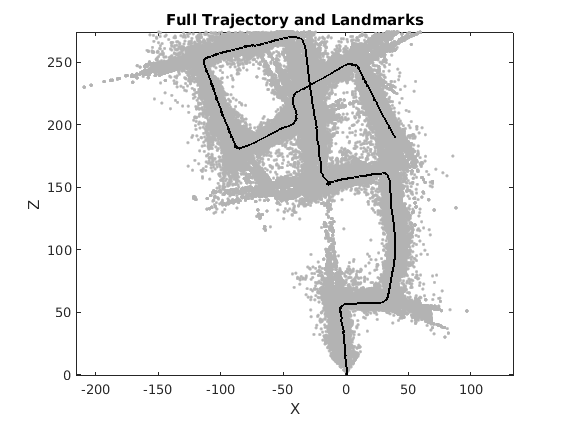
\includegraphics[width=0.6\textwidth]{Results_KITTI.png}
\caption{KITTI dataset full trajectory and landmarks}
\end{figure}

KITTI dataset shows significant scale drift without the bundle adjustment implementation. After bundle adjustment, the VO pipeline is robust enough to run to the end of the dataset. 
\section{Malaga} \label{sec:malaga}
MALAGA dataset shows scale drift even after bundle adjustment. This is thought to be from the large variations of landmark distance from the camera.

\begin{figure}[h]
\centering
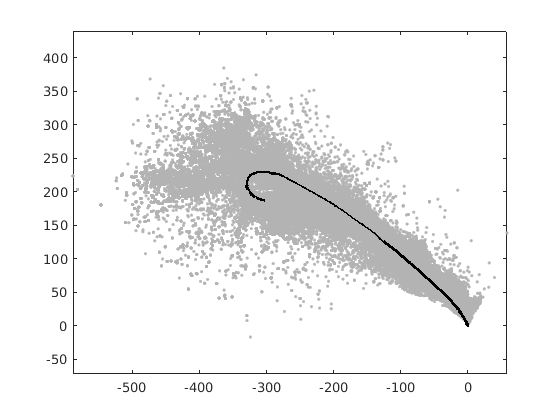
\includegraphics[width=0.6\textwidth]{Results_MALAGA.png}
\caption{MALAGA dataset full trajectory and landmarks}
\label{fig:	results_malaga}
\end{figure}

\section{Parking} \label{sec:parking}
Parking dataset shows robust performance even though the camera is facing the right angle to the direction of travel. Parking has an acculative error as the dataset has no loop even though running bundle adjustment. 

\begin{figure}[h]
\centering
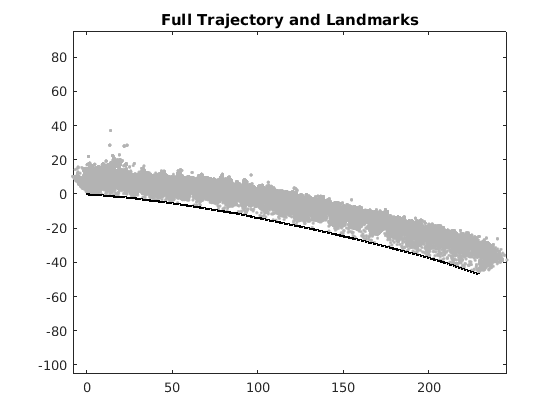
\includegraphics[width=0.6\textwidth]{Results_Parking.png}
\caption{Parking dataset full trajectory and landmarks}
\label{fig:	results_parking}
\end{figure}

\section{Custom Dataset (Seoul)} \label{sec:Custom our_dataset}

A custom dataset was constructed to verify that the visual odometry pipeline is robust enough to work in various environments. The custom dataset is based on 360 sequence of images taken from an iPhone 6s. While taking the images the camera had a fixed focal length and the images were down sampled by a factor of 0.2 for computational issues in calibrating the camera and rectifying images. Images were filmed in a narrow alley in Seoul, Republic of Korea in December 27th 2016.\newline
The successful trajectory estimation of the VO pipeline in a narrow alley with large variations of landmark distance and illumination changes shows robust performance of the VO pipeline.

\begin{figure}[h]
\centering
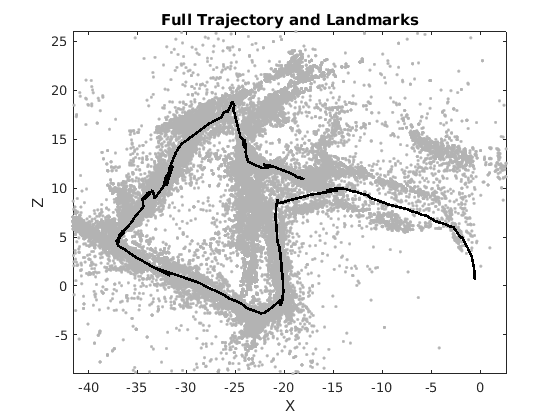
\includegraphics[width=0.6\textwidth]{Results_OWN.png}
\caption{Seoul dataset full trajectory and landmarks}
\end{figure}

\begin{figure}[h]
\centering
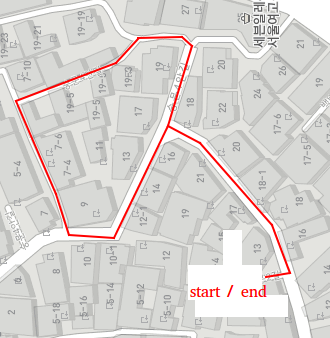
\includegraphics[width=0.5\textwidth]{seoul_ground.png}
\caption{Estimated Ground truth of Seoul dataset from Daum Map}
\end{figure}

\section*{Video Links}

\begin{itemize}
\item Youtube Playlist \url{https://www.youtube.com/playlist?list=PL4osb-habf7AwyqOOP_enbcIkzncwvSIB}
\item KITTI: \url{https://youtu.be/dS4KoISoAcE?list=PL4osb-habf7AwyqOOP_enbcIkzncwvSIB}
\item Malaga: \url{https://youtu.be/3fxA7I47CuM?list=PL4osb-habf7AwyqOOP_enbcIkzncwvSIB} 
\item Parking: \url{https://youtu.be/WfOTkpfoyzY?list=PL4osb-habf7AwyqOOP_enbcIkzncwvSIB}
\item Seoul (our data set): \url{https://youtu.be/Y0lDwR3oK0w?list=PL4osb-habf7AwyqOOP_enbcIkzncwvSIB}
\end{itemize}

\section{Conclusions}
We successfully implemented a fully working and robust monocular visual odometry pipeline as well as the additional features as the following. 

\begin{itemize}
\item An appealing visualization was implemented including keypoint tracking information, camera heading and trajectory in each frame. A full landmark and trajectory visualization is also implemented.
\item Many ideas for improving the performance of the VO pipeline. 
\item refined estimated pose by minimizing reprojection error.
\item VO pipeline verification on a custom recorded dataset.
\item Full bundle adjustment(motion and structure)
\item Not fully working but implemented loop closure module using place recognition. 
\end{itemize}

%\appendix

%\chapter{Dummy Appendix}

You can defer lengthy calculations that would otherwise only interrupt
the flow of your thesis to an appendix.


\backmatter

\bibliographystyle{plain}
\bibliography{refs}

%\includepdf[pages={-}]{declaration-originality.pdf}

\end{document}
